\documentclass[11pt, a4paper]{article}
\usepackage[
        left=0.50in,
        right=0.50in,
        top=1.0in,
        bottom=1.0in,
        paperheight=11in,
        paperwidth=8.5in
]{geometry}
\usepackage{amsmath, amsthm}
\usepackage{amssymb}
\usepackage{verbatim}
\usepackage[export]{adjustbox}
\usepackage{pifont}
\usepackage{array,multirow, rotating}
\usepackage{enumitem}
\usepackage{enotez, multicol}
\usepackage[bottom]{footmisc}
\usepackage{caption, float}
\usepackage{subcaption}
\usepackage{titlesec}
\usepackage{makecell}

\usepackage{tikz}
\usepackage{pgfplots}
    \usetikzlibrary{intersections}
    % create a custom style to store common `axis' options
    \pgfplotsset{
        gstyle/.style={
            xmin=-5,
            xmax=5,
            ymin=-5,
            ymax=5,
            xtick distance=1,
            ytick distance=1,
            axis lines=center,
        },
    }

\usepackage{hyperref}
% \hypersetup{colorlinks=true, pdfstartview=FitV, linkcolor=blue, citecolor=blue, plainpages=false, pdfpagelabels=true, urlcolor=blue}
\usepackage[all]{hypcap}
\usepackage[extrafootnotefeatures]{xepersian}
\usepackage{float}

\newcommand{\risktbl}[3]{
\large #1 \normalsize
\begin{table}[H]
\begin{center}
\caption{احتمال و شدت ریسک}
\begin{tabular}{|c|c|c|}
	\hline
	\textbf{درصد احتمال وقوع} & \textbf{شدت ریسک} \\
	\hline
	#2 & #3 \\
	\hline
\end{tabular}
\end{center}
\end{table}
}

\newcommand{\bt}[1]{\large #1 \normalsize}

\title{پروژه درس تحلیل و طراحی سیستم}
\author{{\textbf{علیرضا ارزه گر}} \\
{\href{mailto:alirezaarzehgar82@gmail.com}
        {\texttt{<alirezaarzehgar82@gmail.com>}}} \\
        {Islamic Azad University, Mashhad}\\
        {مدرس:استاد واحدی}
}
\settextfont[
	Scale=1.4,
	Extension=.ttf,
	Path=ttf/,
	BoldFont=XB NiloofarBd,
	ItalicFont=XB NiloofarIt,
	BoldItalicFont=XB NiloofarBdIt
]{XB Niloofar}
\linespread{2} %regulate line spacing
\begin{document}

\maketitle
\newpage

\tableofcontents
\newpage

\section{پیش گفتار}
در این تحقیق قصد داریم که به تعبیر هندسی مشتق مراتب بالای توابع بپردازیم. فهمیدن این موضوع بسیار به درک مفهوم مشتق کمک خواهد کرد.
از طرفی مشتقات مراتب بالای یک تابع به ما اطلاعات خاصی را از آن تابع خواهد داد. این تحقیق به دنبال این هست که برسی کند مشتق مراتب بالای یک تابع دقیقا چه اطلاعاتی را به ما خواهد داد.
درواقع می‌خواهیم ببینیم مشتق یک تابع چه اطلاعاتی را از منظر هندسه به ما می‌دهد.

\section{مقدمه ای بر پروژه CRM}
با بزرگ تر شدن شرکت و افزایش تسک ها، تیم مدیریت سازمان ما نیاز به سیستمی دارد که بواسطه آن دپارتمان های مختلف سازمان را مدیریت کند.
برای خیلی از کار های مدیریتی همیشه ابزار هایی وجود خواهد داشت. سازمان ما برای مدیریت کار های خود، نیاز به یک CRM شخصی سازی شده دارد.
CRM درواقع سیستمی است که بواسطه آن شرکت خدمات خود را به کارکنان یا حتی مشتری های خود ارائه می‌دهد.
سیستم های زیادی از قبل توسعه داده شده اند که کار تیم مدیریت را تسهیل کنند. اما مشکلاتی وجود دارد که در ادامه مستند به آنها خواهیم پرداخت.
اغلب نیاز های هر سازمان با سازمان دیگری فرق خواهد کرد. این موضوع زمانی که سازمان ها بزرگ تر می‌شوند بیشتر به چشم خواهد آمد.
از همین رو نیاز ها و استاندارد های سازمان مورد نظر شخصی و یکتا تر خواهد شد. در چنین حالتی ما نیاز به سیستم های انعطاف پذیر تری خواهیم داشت.
سیستمی که سازمان ما مدنظر دارد، باید بتواند به تیم مدیریت در اداره دپارتمان های مختلف کمک کند. در این مقدمه به نیاز های کلی دپارتمان های مختلف خواهیم پرداخت.

\subsubsection{نیازمندی های کلی تیم محصول}
تیم محصول نیاز دارد تا با استفاده از متودولوژی اسکرام اسپرینت ایجاد کند و تسک های مربوط به هر اسپرینت را با جزئیات وارد سیستم کند.
ارائه یک برد اسکرام یا کانبان، یا دنبال کردن تسک ها و برسی عملکرد نیرو ها از کلی ترین نیاز های این دپارتمان خواهد بود.

\subsubsection{نیازمندی های کلی تیم حساب داری}
تیم حساب داری نیاز دارد از سیستم منسوخ شده بروکراسی خود فاصله گرفته و به فرایند خودکار ثبت ورود، خروج و محاسبه حقوق کارمند ها روی بیاورد.
نیاز کلی سازمان حذف بروکراسی و بایگانی دقیق و بی نقص اطلاعات بواسطه خودکار سازی فرایند های حسابداری است.

\subsubsection{نیازمندی های کلی تیم فنی}
تیم فنی علاوه بر برسی فعالیت های خود بر روی برد اسکرام، نیاز دارد در محیطی مستندات فنی خود را قرار بدهد. چنین بستری باید دارای سطوح دسترسی مختلف باشد.
ایجاد فضا های مختلف و نوشتن مستندات فنی مرتبط با پروژه های مختلف یکی از قابلیت های الزامی ای هست که تیم فنی به آن نیاز خواهند داشت.
علاوه بر آن، تیم فنی نیاز دارد یک سری از گزارشات را هم دنبال کند. برای مثال گزارشات تیم SRE یا تیم امنیت باید برای تیم فنی قابل رویت باشد.

\subsection{براورد هزینه ها}
همانطور که اشاره کردیم، ابزار های بسیاری از قبل توسعه یافته اند تا کار تیم های مختلف را ساده کنند. اما تمامی آنها رایگان نیستند.
نمونه ابزار هایی که می‌توان استفاده کرد را ذکر می‌کنیم.

\begin{itemize}
	\item تیم حساب داری برای برسی ورود و خروج کارمندان می‌تواند از نرم افزار KaraWeb استفاده کند.
	\item تیم مدیر محصول برای استفاده از متودولوژی اسکرام می‌تواند از نرم افزار پرمیوم جیرا استفاده کند.
	\item تیم توسعه نرم افزار و باقی تیم های فنی برای نگه داری کد ها و مستندات می‌توانند از GitLab استفاده کنند.
\end{itemize}

در مثال هایی که قید کردیم، کاراوب و جیرا هردو نیاز به پرداخت هزینه دارند.
برای مثال فقط نرم افزار جیرا مبلغی حدود 15250 دلار برای اشتراک سالانه نسخه پرمیوم خود اخز می‌کند. چیزی حدود ۷۰ میلیون تومان در تاریخ نوشته شدن این سند.
با محاسبه این هزینه ها و نیازمنان، باید براورد کنیم که چه کاری درست خواهد بود ؟
آیا توسعه یک سیستم شخصی CRM صرفه اقتصادی می‌کند ؟

\subsubsection{برسی هزینه ها و سود پروژه}
همانطور که اشاره کردیم، برای خرید ابزار های مورد نیاز سالیانه حدود ۸۰ میلیون کمپانی باید هزینه کند. از بین این هزینه ها، خیلی از فیچر ها بلا استفاده بوده
و خیلی از خواسته ها براورده نخواهند شد.
کمپانی چند نیرو با مبلق قانون کار دارد و با درنظر گرفتن قانون کار ۱۰ میلیون، اگر ۳ کارمند به طور تمام وقت کار کنند، اگر قبل از ۲ ماه پروژه به پایان برسد شرکت سود کرده است.
هرچند اگر این زمان بیشتر بشود باز هم شرکد در ضرر نیست. چرا که این سیستم محدود به یک سال نخواهد بود.
علاوه بر آن پس از توسعه این سیستم، می‌توانیم آن را به شرکت های دیگر نیز ارائه دهیم و درامد مضاعفی از فروش اشتراک ها یا پلاگین های آن داشته باشیم.
پس حتی تعداد بیشتری می‌توان روی این پروژه کار کند و این پروژه علاوه بر اینکه نیاز های شرکت را برطرف می‌کنید، خود منبع درامد نیز خواهد بود.

بنا بر این برنامه ما توسعه یک سیستم کامل CRM خواهد بود که نیاز های داخلی خود و دیگران را رفع بکند.
برای اینکار نیاز خواهیم داشت که طراحی ماژولار داشته باشیم و سیستم بر اساس نیاز کاربر تنظیم بشود.

\newpage
\section{مدل مورد استفاده در توسعه سیستم}
سیستمی که می‌خواهیم توسعه دهیم نیازمند فرایند های رفت و برگشتی بسیاری بین عوامل مختلف روند توسعه محصول هست. از ساعتی که پروژه شروع به توسعه می‌کند، 
نیازمندیم مرحله به مرحله کار ها رو به ترتیب اولویت انجام دهیم و به صورت چرخشی بازگردیم. برای مثال در نسخه اولیه که میخواهیم ارائه دهیم، دقیق نمیدانیم راهکار هایی که
در ذهن داریم، آیا جوابگو نیاز های کاربران هست یا خیر. از طرفی باگ ها و مشکلاتی در آینده وجود خواهند داشت که درحال حاضر از آنها بی اطلاع  هستیم.
جنبه های بیزینسی نیز کم نخواهند بود. به احتمال خیلی زیاد بعد از انتشار نسخه MVP ایراداد بیزینسی زیادی به پروژه وارد خواهد شد و این مشکلات به مرور زمان
در جلسات طراحی نرم افزار و بیزینس لاجیک باید صحبت بشوند. محصول نیاز به چندین بار طی کردن روند توسعه نرم افزار خواهد بود.

برای اینکه دقیق تر به موضوع بپردازیم، مرحله به مرحله قید خواهیم کرد. در مرحله اول، تیم UX باید تحقیق کنند که چه چیز هایی برای سیستم CRM ما نیاز هست.
باید ذی‌نفعان این محصول را شناسایی کرده و با تمامی آنها جلسه ای تنظیم کرد. پس از صحبت با آنها، می‌توان معماری بهتری چید.
برای مثال تیم محصول، حساب داری و فنی می‌توانند نظرات مفیدی را درمورد نیاز های خودشان بیان بکنند. این نظرات باید بایگانی شوند تا بعدا در جلسات طراحی برای 
رفع آنها فکر شود. البته در صورتی که درخواست ها منطقی باشند.
پس از آن تیم معماری نرم افزار (Architects) بر ساس یافته های خود شروع به چیدن یک سیستم می‌کنند.

بعد از مشخص شدن سیستم و شکوندن تسک ها و بستن اسپرینت توسط مدیر محصول، تیم های فنی دست به کار می‌شوند. توسعه دهنده ها شروع به نوشتند اجزا اصلی 
سیستم می‌کنند. تیم operation محیت لازم برای توسعه دهنده ها فراهم می‌کند.
تیم DevOps فرایند های اوتوماسیون لازم را می‌چیند و مهندسین تست انواع تست ها را مشخص می‌کنند.

نرم افزار داخل محیط تستی لانچ شده و تست می‌شود. بعد از گرفتن تائید واحد کنترل کیفیت، به مرحله بعد می‌رویم.

محصول بدست آمده به بازار ارزه می‌شود و بر اساس فیدبک ها و مشکلات گزارش شده تصمیم گرفته می‌شود که این چرخه ادامه داشته باشد یا خیر.

مدل توسعه نرم افزاری که این سیستم نیاز دارد، مدل توسعه مارپیچی خواهد بود. چرا که چندین مرحله به فیدبک گیری نیازمند خواهیم بود.

\subsection{مدل مارپیچی}
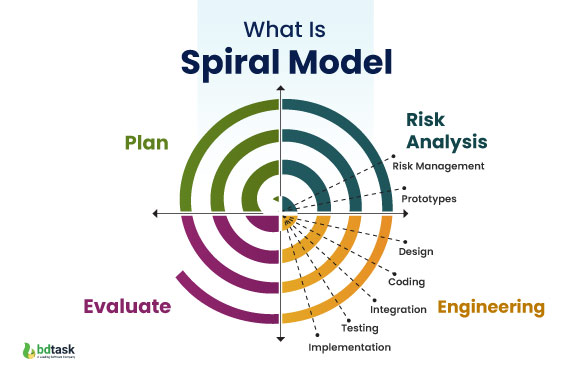
\includegraphics{assets/spiral_model.jpg}


\newpage

\section{برنامه ریزی}
در این بخش به برسی موجودیت های کلی سیستم و PRD های نسخه اولیه سیستم می‌پردازیم.

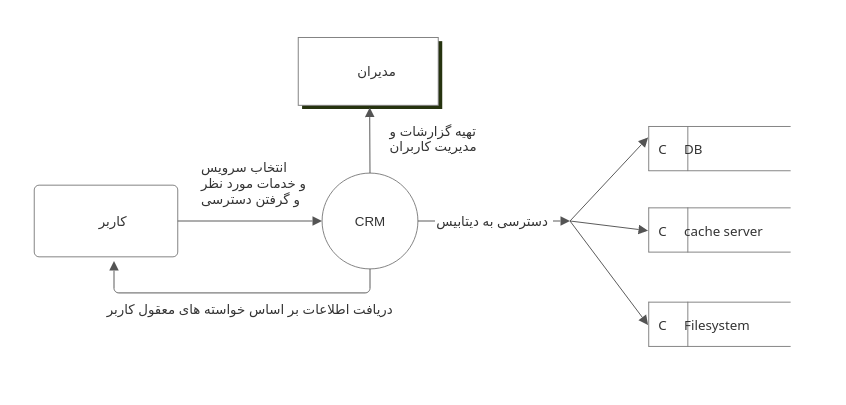
\includegraphics[scale=0.8]{assets/0_level_system.png}

سیستم سطح صفر، و انتزاعی ترین مدل سیست به صورت نمودار DFD فوق است.
کاربر وارد سیستم شده و بر اساس سطوح دسترسی خود حق انتخاب سرویس های مورد نظر خود را خواهد داشت. بعد از آن
داده های خود را بواسطه سیستم در دیتابیس های مختلفی می‌تواند ذخیره کند.
برای مثال رکورد های دیتابیس در Postgres ذخیره شده، برخی لاگ ها یا رویداد ها بواسطه Redis منتقل شده و مستندات بصورت فایل داخل سرور قرار می‌گیرند.

در کنار این روند کلی، مدیران سطوح بالا تر و خود کاربران می‌توانند داده های بسیاری را در سیستم مشاهده کنند.

سیستم به زیر سیستم های مختلفی تقسیم می‌شود که به آنها خواهیم پرداخت.

\subsection{زیر سیستم احراز هویت}
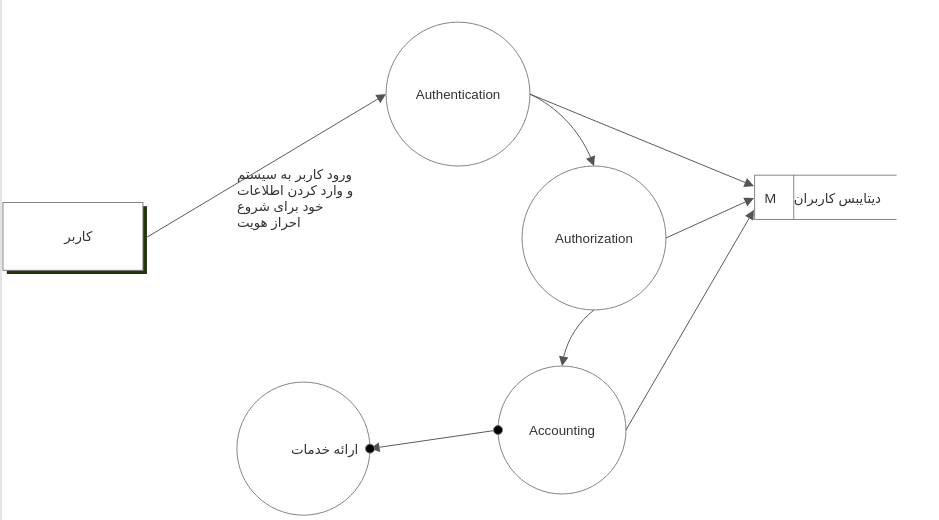
\includegraphics[scale=0.8]{assets/auth_dfd.png}

نمودار DFD مرتبط با احراز هویت کاربران به این شکل می‌باشد.
مراحل احراز هویت با جزئیات بیشتر توضیح داده خواهد شد:

\begin{itemize}
	\item کاربر ابتدا مشخصات خود را در سیستم وارد می‌کند.
	\item سیستم طی مرحله ای به نام Authentication تشخیص می‌دهد که آیا کاربر اجازه ورود به سیستم دارد یا خیر.
	\item بعد از آن سیستم در مرحله Authorization مشخص می‌کند که کاربر به چه بخش هایی از سیستم می‌تواند دسترسی داشته باشد.
	\item بخش دیگری از سیستم با نام Accounting در حین استفاده کاربر از سیستم، گزارشاتی را طهیه خواهد کرد و برای مدیریان سطح بالا تر ارسال می‌کند.
	\item در نهایت نیز کاربر می‌تواند به سرویس دلخواه و قابل دسترس خود دست پیدا کند.
\end{itemize}

در نمودار ERD زیر به موجودیت ها و صفات موجود در کاربر ها و role هایشان می‌پردازیم.

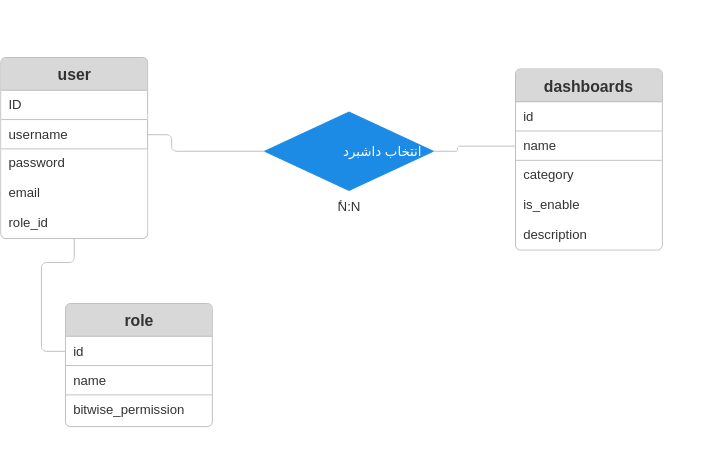
\includegraphics[scale=0.8]{assets/auth_erd.png}

همانطور که مشاهده می‌کنید، هر کاربر یک role دارد. این مقادیر را سیستم در حین احراز هویت از دیتابیس دریافت کرده و بر اساس آن انتخاب می‌کند
کدام کاربر حق ورود به چه زیر سیستم هایی را دارد.

\subsection{زیر سیستم حساب داری}

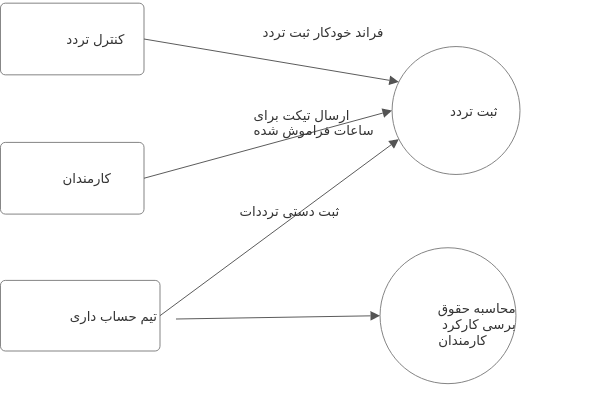
\includegraphics[scale=0.8]{assets/finance_dfd.png}

زیر سیستم حساب داری دو وظیفه مهم را بر عهده دارد. تیم های مختلف می‌توانند از طریق این زیر سیستم تردد و گزارشات مرتبط به آن را دنبال کنند.
روزانه کارمندان بواسطه دستگاه تردد، ورود و خروج های خود را ثبت می‌کنند.
این سیستم به دستگاه ثبت تردد متصل بوده و این تردد ها را به صورت خودکار داخل دیتابیس ثبت خواهد کرد.
در صورتی که فرد فراموش کرده بود، می‌تواند به مدیران حساب داری و منابع انسانی اطلاع دهد. این مدیران به صورت مستقیم
توانایی و اجازه ویرایش و اضافه کردن رکورد به دیتابیس ورود و خروج دارند.
راه دیگر آنها نیز تیکت زدن به واحد مدیریت خواهد بود.

زیر سیستم حساب داری بیشتر خدمات خود را به واحد منابع انسانی خواهد داد. به طوری که در داشبرد منابع انسانی، می‌تواند برای کارمندان
حقوق و الگوریتم محاسبه آن تعریف شود. در کنار آن گرفتن مرخصی و بثبت پرداختی ها از همین بخش انجام خواهد شد.

\subsection{زیر سیستم مدیریت پروژه}
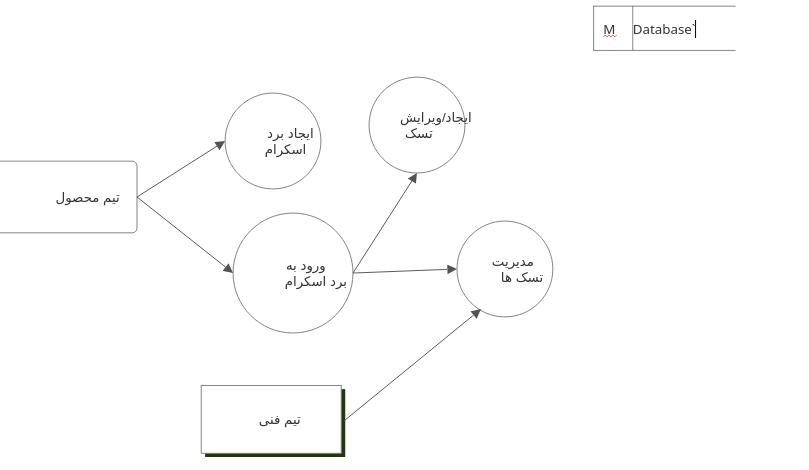
\includegraphics[scale=0.8]{assets/product_dfd.png}

تیم محصول می‌تواند برد های مورد نیاز خود را ایجاد کند و تسک های لازم را برای بستتن اسپرینت ها و استفاده از اسکرام تعریف کند.
تیم فنی نیز می‌تواند تسک های خود را دنبال کند، و وضعیت آنها را بر اساس آنچه که باید تغییر بدهد. تیم فنی باید تخمین های زمانی و زمان سپری کرده روی هر تسک را 
در این زیر سیستم مشخص کند.
تیم فنی و محصول هر  زمان بخواهند می‌توانند گزارشات مرتبط با عملکرد کاری خود را مشاهده کنند.
اما تیم محصول گزارشات بیشتری خواهند داشت.
برای مثال اگر توسعه دهنده ای بیش از حد تسک هایی داشته باشد که زمان سپری شده آنها بیش از زمان تخمین زده باشد، به مدیر محصول اخطار داده می‌شود.
تمام داده ها در دیتابیس ذخیره شده و مجددا می‌تواند مورد استفاده قرار گیرد.

\subsection{زیر سیستم مستند سازی}
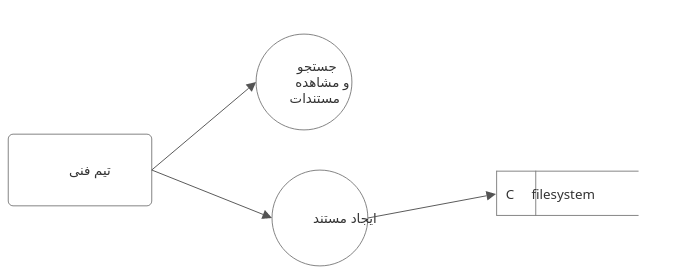
\includegraphics[scale=0.8]{assets/doc_dfd.png}

تیم فنی می‌تواند بر اساس دسترسی خود مستنداتی بسازد و باقی تیم نیز بر اساس سطوح دسترسی به مستندان فنی مختلف دسترسی داشته باشند.
نکته حائز اهمیت در این سیستم، امنیت و سطوح دسترسی آن خواهد بود. مدیران بالا تر می‌توانند دسته بندی و پروژه های مختلف تعریف کنند و به نیرو های دیگر
بر اساس نیاز دسترسی های مختلف بدهد.
کاربر می‌تواند فقط دسترسی دیدن مستندات خاصی را داشته باشد یا بتواند آنها را ویرایش یا حذف کند.

ادمین و سازنده هر مستند می‌تواند لیست افرادی که به آن دسترسی دارد را کنترل کند. این لیست درواقع به جدول role مرتبط است که قبل تر به آن اشاره شده.

\subsection{زیر سیستم مدیریت تنظیمات}
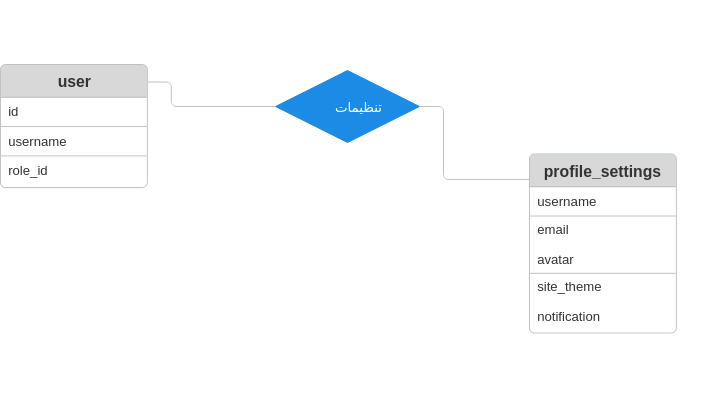
\includegraphics[scale=0.8]{assets/settings_erd.png}

کاربرات از بخش تنظیمات می‌توانند اطلاعات کلی حساب کاربری خود را ویرایش کنند. از این بخش، نام، ایمیل و عکس پروفایل خود را می‌توانند تغییر دهند.
همچنان تم سایت و اینکه نوتیفیکیشن ارسال بشود یا خیر قابل تنظیم است.

\subsection{زیر سیستم مانیتورینگ}
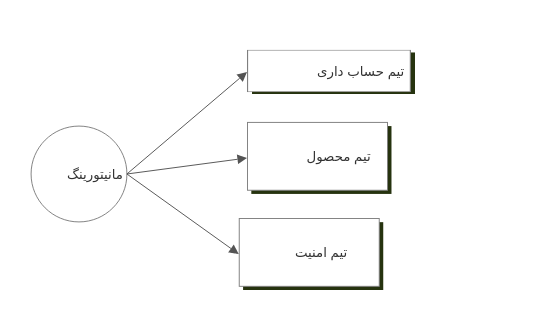
\includegraphics[scale=0.8]{assets/monitoring_dfd.png}

رخداد ها و اتفاق هایی در سیستم وجود دارد که سیستم می‌تواند آنها را به کاربران اعلان کند و از مشکلات و اتفاقاتی خبر دار کند.
سیستم مانیتورینگ به هر دسته و سطوح دسترسی خاص، بر اساس وظایف آنها یک سری لاگ ها و اعلان ها را ارسال می‌کنید.

\subsubsection{اعلان های سیستم مانیتورینگ برای تیم حساب داری}
\begin{itemize}
	\item غایب بودن یک نیرو خاص
	\item وجود کسری کار غیر معقول برای یک شخص
	\item دیر شدن در پرداختی های کارمند ها 
\end{itemize}

\subsubsection{اعلان های سیستم مانیتورینگ برای تیم محصول}
\begin{itemize}
	\item نرسیدن تسک ها با اسپرینت
	\item ثبت غیر معقول زمان سپری شده روی یک تسک برای کاربری خاص
	\item گزارشات ناقص یک کاربر
	\item تغییر مثبت و منفی یک نیرو در بازه زمانی خاص
\end{itemize}

\subsubsection{اعلان های سیستم مانیتورینگ برای تیم امنیت}
\begin{itemize}
	\item تلاش کاربر نا شناخته برای ورود به سیستم
	\item محدود بودن منابع سرور و خطر
	\item حمله ای از سمت یک کاربر ناشناخته درحال انجام است
\end{itemize}


\section{مدیریت ریسک ها}

\subsection{شناسایی ریسک ها}
تهدیدات و ریسک های مختلفی پروژه CRM را تحدید خواهند کرد که باید از قبل برای آنها چاره اندیشی کرده باشیم.
انواع مختلف ریسک ها می‌تواند گریبان گیر پروژه باشد. در این مرحله به برسی و شناسایی ریسک های مختلف خواهیم پرداخت.

انواع خطر هایی که می‌تواند سیستم CRM را تهدید کند، با دسته بندی می‌نویسیم.

\subsubsection{آسیب پذیری سخت افزار}
در هر برهه زمانی ای ممکن است سخت افزاری که اپلیکیشن بر روی آن است دچار مشکل بشود. در لیست زیر مثال هایی از مشکلات سخت افزاری و زیر ساختی قید می‌شود.

\begin{itemize}
	\item خرابی سرور پروداکشن
	\item رفتن برق دیتاسنتر
	\item سوختن حافظه سرور دیتابیس
	\item اختلال در شبکه دیتاسنتر
\end{itemize}

\subsubsection{آسیب پذیری نرم افزار}
در صورتی که سخت افزار سالم باشم، ریسک ها و مشکلاتی وجود دارد که می‌تواند در سمت نرم افزاری محصول رخ بدهد. در لیست زیر به شناسایی این مشکلات می‌پردازیم.

\begin{itemize}
	\item وجود انواع باگ های عملکردی در سیستم و ایجاد اختلال
	\item حملات DoS
	\item پر شدن ترافیک سرور
	\item ایجاد کانفلیکت در فرایند دیپلوی کردن نرم افزار و خرابی موقت سیستم
	\item مورد حمله قرار گرفتن سیستم
\end{itemize}

\subsubsection{آسیب پذیری اپراتور}
گاهی سخت افزار و نرم افزار سالم بوده، اما اپراتور دچار مشکل می‌شود. برای مثال اشکالات احتمالی زیر را خواهیم داشت.

\begin{itemize}
	\item اشتباه وارد کردن ورود و خروج
	\item فراموشی ثبت
	\item چیدن اشتباه برد های اسکرام توسط مدیر محصول
	\item عدم وارد کردن زمان سپری شده توسط نیرو های فنی
	\item ایجاد خرابی عمدی توسط یک کاربر با دسترسی خاص
\end{itemize}

\subsection{تحلیل و دسته بندی ریسک ها}
مشکلات و ریسک های احتمالی را در نسخه MVP سیستم شناسایی و دسته بندی کردیم. حال نوبع تحلیل آنها و برسی این است که هر ریسک چقدر احتمال وقوع دارد
و چقدر می‌تواند آسیب بزند. این مورد بسیار حائز اهمیت است.

\subsubsection{آسیب پذیری سخت افزار}
به مراتب احتمال وقوع مشکلات سخت افزاری نسبت به ریسک های دیگر کمتر است. اما اگر آن را نسبت به زمانی که سیستم مورد استفاده قرار می‌گیرد
و خساراتی که به سیستم می‌زند بسنجیم، متوجه می‌شویم بسیار مهم است. درصد کمی احتمال دارد یک مشکل سخت افزاری در این سیستم رخ بدهد. اما فرضا در طول ۱۰ سال
استفاده یک مشتری از این سیستم، یک درصد احتمال هم به معنی بار ها اتفاق افتادن مشکل هست.

\risktbl{خرابی سرور پروداکشن}{>1\%}{غیر قابل تحمل}

مثال های زیادی وجود دارد که در آن سرور پروداکشن دچار مشکل می‌شود. برای مثال ممکن است به هر دلیلی یکی از اجزا اصلی سرور دچار مشکل شود.
مثلا RAM یا CPU سرور خراب شود. در این حالت تیم Operation باید چاره اندیشی کند و به فکر این مشکل باشد که زمان و هزینه زیادی مصرف خواهد شد.

\risktbl{رفتن برق دیتاسنتر}{>10\%}{حداقل بودن ریسک}

رفتن برق دیتاسنتر ها گاها اتفاق میوفتد و دور از انتظار نخواهد بود. تیم فنی و Operation باید به دنبال راهکاری باشند که چنین مشکلی پیش نیاید.

\risktbl{خرابی حافظه سرور دیتابیس}{>1\%}{غیر قابل تحمل}

به هر دلیلی ممکن است Storage سرور پروداکشن یا دیتابیس دچار مشکل شده و تمام داده ها از بین برود. تیم فنی باید راهکاری پیدا کند که در صورت وقوع چنین حادثه ای،‌
دیتا کاربران از بین نرود.

\risktbl{اختلال در شبکه دیتاسنتر}{>1\%}{غیر قابل تحمل}

در مواقعی شبکه داخلی یک سازمان یا دیتاسنتر دچار مشکل می‌شود. در این حالت مدیران فنی به سرعت باید مشکل را کشف و حل کنند.

\subsubsection{آسیب پذیری نرم افزار}
بر خلاف مشکلات سخت افزاری، مشکلات نرم افزاری بسیار احتمال وقوع بیشتری دارند و حتی می‌توانند هزینه بیشتری را به دوش شرکت بیندازند. 

\risktbl{وجود انواع باگ های عملکردی در سیستم و ایجاد اختلال}{>20\%}{حداقل بودن ریسک}

باگ ها و مشکلات نرم افزاری همیشه بودند. اما در صورتی که به سادگی بتوان از آنها سو استفاده کرد و تعداد آنها بسیار زیاد باشد، سیستم دچار مشکل بزرگی می‌شود.
تمام تلاش تیم توسعه نرم افزار باید این باشد که محصولی توسعه بدهد که کمترین باگ ممکن را داشته باشد.

\risktbl{حملات DoS}{>10\%}{غیر قابل تحمل}

در صورتی که سیستم دچار حمله DoS بشود، کاربران دیگر نمی‌توانند برای مدتی از سرویس استفاده بکنند. این مشکلی به شدت جدیست که باید از سمت
تیم Operation و Security چاره اندیشی بشود.

\risktbl{پر شدن ترافیک سرور}{0\%}{قابل قبول}

یک سیستم داخلی CRM بعید است بخاطر ترافیک زیاد داون شود. از این رو. به همین دلیل نیازی به نگرانی از این بابت نخواهد بود. در صورتی که سیستم در گستره بزرگ تری
مورد استفاده قرار گیرد نیز نیاز به تدابیر بیشتری خواهد داشت.

\risktbl{ایجاد مشکل در فرایند دیپلوی کردن نرم افزار}{<30\%}{حداقل بودن ریسک}

زمانی که نسخه جدید از نرم افزار توسعه پیدا می‌کند، مشکلاتی برای دیپلوی کردن آن نسخه اتفاق خواهد افتاد. برای مثال ممکن است  نسخه دیپلوی شده باگ داشته باشد
یا حتی تیم Operation نتواند به درستی آن را Deploy کند. در این حالت باید از تیم های DevOps کمک گرفت. در این حالت احتمال مشکل در فرایند Deployment
کمتر و کمتر خواهد شد.

\risktbl{مورد حمله قرار گرفتن سیستم}{>20\%}{غیر قابل تحمل}

همواره کسانی وجود دارند که با نیت های مختلف علاقمند هستند به سازمان ها نفوذ کنند. سیستم CRM ما نیز از این خطر دور نیست. من باب رفع خطر، باید از تیم فنی و امنیت 
کمک گرفته شود و تدابیری صورت بگیرد.

\subsubsection{آسیب پذیری اپراتور}
در صورتی که سیستم به درستی طراحی نشود، اپراتور ها سهوا یا عمدا می‌توانند به سیستم آسیب بزنند. در جدول فوق به برسی این ریسک ها خواهیم پرداخت.

\risktbl{اشتباه وارد کردن ورود و خروج}{<30\%}{قابل قبول}

خطای انسانی بسیار رایج بوده و هیچ زمان نمیتوان آن را به صفر رساند. در موارد زیادی ممکن است کاربر و مدیران داده های اشتباهی به سیستم ارائه دهند.
این مشکل باید از طریق طراحی درست سیستم حل بشود.

\risktbl{فراموشی ثبت}{<50\%}{قابل قبول}

خیلی از موارد کاربر فراموش خواهد کرد از دستگاه کنترل تردد استفاده کند. در این حالت به واسطه طراحی مناسب سیستم می‌توان به مدیر درخواست داد یا تیکت زد.
این ریسک نیز قابل قبول بوده و به راحتی قابل حل است.

\risktbl{چیدن اشتباه برد های اسکرام توسط مدیر محصول}{>10\%}{قابل قبول}

اشتباه در چیدن برد اسکرام شرکت را متحمل ضرر زیادی نخواهد کرد. احتمالا با چند بار review ساده کار قابل مشاهده باشد. اما باز هم تیم فنی می‌تواند سیستم را طوری طراحی کند 
که کاربران از ساختاری استاندارد پیروی کنند.

\risktbl{عدم وارد کردن زمان سپری شده توسط نیرو های فنی}{<40\%}{حداقل بودن ریسک}

ممکن است نیرو ها سهوا یا عمدا برای تسک های خود زمان سپری شده را ثبت نکنند یا اشتباه وارد کنند. در این حالت سیستم باید طوری طراحی شود که این 
اتفاق کمتر رخ بدهد یا رخ ندهد.

\risktbl{ایجاد خرابی عمدی توسط یک کاربر با دسترسی خاص}{>5\%}{غیر قابل تحمل}

این مشکل تهدید بزرگی است. برای رفع آن تیم فنی باید به درستی سطوح دسترسی را تنظیم کند.

\subsection{براورد و کاهش هزینه حاصل از ریسک ها}
در این مرحله باید ریسک هایی که شناسایی کردیم و تحلیل کردیم را برطرف کنیم و برای آنها راهکار ارائه دهیم.
این راهکار ها باید عملیاتی و نرم افزاری باشند.

\subsubsection{آسیب پذیری سخت افزار}
رفع مشکلات سخت افزاری و چاره اندیشی برای آنها هزینه مشکلات زیادی به همراه دارد و هزینه بر تر از کار های دیگر است. بهرحال تدابیری را درنظر خواهیم گرفت.

\bt{خرابی سرور پروداکشن:}
برای جلوگیری از خرابی سرور های پروداکشن باید مرتبا سیستم ها مانیتور شوند. نیازداریم با ابزار هایی نظیر Grafana و Prometheus برسی کنیم که در هر لحظه
آیا سرور ها عملکرد مناسبی دارند یا خیر ؟
در صورتی که مشکلی مشاهده شد، سریعا باید برطرف شود تا جدی تر نشود.

\bt{رفتن برق دیتاسنتر:}

برای این مشکل می‌توان از UPS استفاده کرد و تا مدتی برق را برای دیتاسنتر تامین کرد. اینطور تا حدی احتمال و خطر رفتن برق دیتاسنتر ها کمتر می‌شود.

\bt{سوختن حافظه سرور دیتابیس:}

در صورتی که Storage سرور ها به مشکل بخورد ما داده های زیادی را از دست خواهیم داد. برای اینکه داده از دست ندهیم، می‌توانیم از فایل سیستم هایی نظیر RAID و این تیپ
مدل ها استفاده کنیم و داده ها را در Storage های مختلف قرار بدهیم. اگر یکی از آنها سوخت، حتما Backup از آن داشته باشیم.

\bt{اختلال در شبکه دیتاسنتر:}

برای این مورد شبکه دیتاسنتر باید مرتبا مانیتور شود و حدالامکان از تغییرات بر روی آن اجتناب شود. اگر هم بنا بر تغییر است، به شدت تست انجام گیرد و 
مطمعن شویم مشکلی در شبکه ایجاد نمیکند.

\subsubsection{آسیب پذیری نرم افزار}
جلوگیری از ریسک های ناشی از مشکلات نرم افزاری عموما به طراحی تیم توسعه و تدابیر امنیتی تیم امنیت باز خواهد گشت.

\bt{وجود انواع باگ های عملکردی در سیستم و ایجاد اختلال:}

برای اینکه مطمعن شویم اپلیکیشن به درستی کار می‌کند، قبل از Release و Deploy کردن پروژه باید تست های مختلفی از سیستم صورت گیرد.
این تست ها را در مراحل جلو تر شرح خواهیم داد. در کنار تست ها، کاربر ها باید به حداقل آپشن هایی که نیاز دارند دسترسی داشته باشند.
نباید به کاربری بیش از نیازش دسترسی دهیم.

\bt{حملات DoS:}

برای رهایی از حملات DoS می‌توان از انواع Firewall های سخت افزاری و نرم افزاری استفاده کرد. یکی از روش هایی که این مشکل را برطرف می‌کند،استفاده 
از API Gateway هایی نظیر Kong می‌باشد.
اینطور که یک IP Whitelist درست می‌کنیم و فقط کاربران مجاز را به آن معرفی می‌کنیم.
پس از این هیچ کس غیر از آن کاربر ها نمیتواند کاری کند و هر بسته ای که ارسال شود به اصطلاح Drop خواهد شد.

\bt{پر شدن ترافیک سرور:}

به دلیل داخلی بودن سیستم CRM و کم بودن تعداد کاربران چنین ریسکی عملا وجود نخواهد داشت.
اما در صورت وجود چنین ریسکی، می‌توان از Load Balancer ها و Proxy Server ها استفاده کرد.
برای مثال NGINX یا HAProxy گزینه مناسبی خواهد بود.
نود های مختلف اپلیکیشن نیز با ابزاری مانند Kubernetes می‌تواند کلاستر و مدیریت شوند.

\bt{ایجاد کانفلیکت در فرایند دیپلوی کردن نرم افزار و خرابی موقت سیستم:}

در صورتی که تیم DevOps وجود داشته باشد و به درستی فرایند ها و pipline ها را بچیند، چنین مشکلی پیش نخواهد آمد.
زیرا فرایند Deployment خودکار بوده و نیازمند پاس شدن تست های مختلف خواهد بود.

\bt{مورد حمله قرار گرفتن سیستم:}

با استفاده از WAF هایی مانند ModSecurity یا NAXI و پیکره بندی آن بر روی اپلیکیشنی مانند NGINX دیگر چنین مشکلی به اندازه قبل وجود نخواهد داشت.
البته باید توجه داشته باشید ابزاری مانند ModSecurity باید به درستی کانفیگ شود. در غیر این صورت عملکرد False Positive خواهد بود گاها.

\subsubsection{آسیب پذیری اپراتور}
برای رفع مشکلاتی که اپراتور ها میتوانند ایجاد کنند، کافیست دیزاین بهتری داشته باشیم.

\bt{اشتباه وارد کردن ورود و خروج}

ورود و خروج هر فرد ابتدا به ساکن از دستگاه کنترل تردد گرفته می‌شود. مدیر ها در صورت صلاح دید می‌توانند این مقادیر را اصلاح کنند.
در صورتی که کارمندی فراموش کند ورود یا خروج بزند، می‌تواند به مدیران سطح بالا تر تیکت بزند و مشکلش رو مطرح کند. در این حالت با تائید مدیر رکورد مناسب ثبت خواهد شد.
برای همین چنین مشکلی در سیستم CRM ما وجود نخواهد داشت.

\bt{فراموشی ثبت}

در صورتی که کاربری فراموش کند ورود یا خروجی بزند، زیر سیستم مانیتورینگ CRM به مدیران سطوح بالاتر اعلام می‌کند که چنین اتفاقی افتاده است.
این اعلان برای خود کاربر هم می‌رود و به همین ترتیب با اطلاع داشتن دو سمت ماجرا، بالاخره داده ای که باید ثبت خواهد شد.

\bt{چیدن اشتباه برد های اسکرام توسط مدیر محصول}

برای ایجاد برد های اسکرام می‌توان Wizard ایجاد کرد تا مدیر محصول بر اساس استاندارد تعریف شده برد ایجاد کند.

\bt{عدم وارد کردن زمان سپری شده توسط نیرو های فنی}

سیستم مانیتورینگ CRM به نیرو های فنی ای که تسک های خود را به درستی زمان بندی نمی‌کنند اعلان می‌دهد و از آنها درخواست می‌کند که زمان سپری شده خود را وارد کنند.
علاوه بر این بدون وارد کردن زمان سپری شده، نباید تسکی Done شود. 

\bt{ایجاد خرابی عمدی توسط یک کاربر با دسترسی خاص}

با چیدن درست سطوح دسترسی برای کاربران، کاربران اجازه ندارند فرا تر از دسترسی خود کاری انجام بدهند. همین برای این موضوع کافی خواهد بود و دیگر با چنین مشکلی در
سطوح بالا تر مواجه نخواهیم بود.


\newpage

\section{توسعه و اعتبار سنجی}
پس از برنامه ریزی و طراحی کردن کلیات نرم افزار، و تحلیل ریسک ها، حال می‌توانیم به پیاده سازی و اعتبار سنجی سیستمی که قصد پیاده سازی آن را داریم بپردازیم.
در این مرحله شروع دیزاین، طراحی و تست اپلیکیشن بر اساس مدل آبشاری می‌پردازیم.

\subsection{تشریح مدل آبشاری}
در این مدل ما یک سری مراحل را به ترتیب انجام داده و فیدبک آنها را به مرحله بعد خواهیم داد. مراحل به شرح زیر خواهند بود:

\begin{enumerate}
	\item تحلیل و تعریف خواسته ها،
	\item طراحی جزئیات نرم افزاری
	\item پیاده سازی و تست واحد
	\item جامعیت و تست سیستم
	\item بکار گیری و نگه داری
\end{enumerate}

\newpage

\subsection{تحلیل و تعریف خواسته ها}

\subsubsection{خواسته های سازمان}
\subsubsection{خواسته های محصول}
\subsubsection{خواسته های کاربر}


\subsection{طراحی سیستم و نرم افزار}
طراحی های کلی نرم افزار در مقدمه و مشخص سازی خواسته ها صحبت شده. الباقی کار نیازمند مشخص سازی و طراحی تیم فنی است. این مستندات از تیم فنی بعد از 
برگزاری جلسات معماری اخز شده و بایگانی می‌شود.
مستندات مربوط به معماری پیاده سازی حدالامکان نباید تغییر کند.

% \subsection{مشخص سازی زیر سیستم ها}

% ERD & DFD %

% \subsection{تهیه الزامات}

\subsection{زمانبندی پروژه}
با مشخص شدن نیازمندی ها و زیرسیستم ها می‌توانیم گانت چارت ارائه دهیم و مشخص کنیم تا کی باید پروژه به اتمام برسد و چه کار هایی را به طور همزمان می‌شود انجام داد.

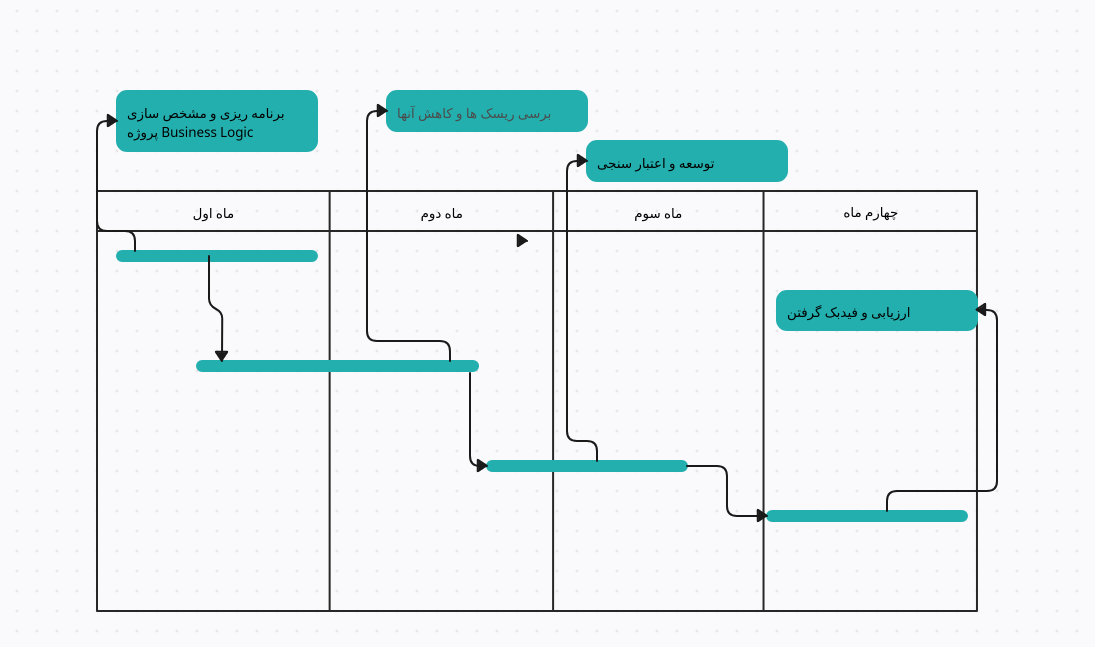
\includegraphics[scale=0.4]{assets/gantt_chart.png}

تلاش بر این است که پروژه بعد از ۴ ماه به خروجی MVP رسیده و به دست مشتری برسد. پس از آن بر اساس مدت پیچشی تا زمانی که محصول می‌تواند بهتر باشد
و صرفه اقتصادی دارد، به توسعه آن ادامه خواهیم داد.

\subsection{راهکار های نظارتی}

\subsection{توسعه سیستم و نرم افزار}

\documentclass[11pt, oneside]{article}
\usepackage[a4paper,left=2cm,bottom=2.5cm,right=2cm,top=2.5cm,footskip=1cm]{geometry}
\usepackage{amsmath, amsthm}
\usepackage{amssymb}
\usepackage{verbatim}
\usepackage[export]{adjustbox}
% \usepackage{fontspec}
% \usepackage{fontawesome}
\usepackage{pifont}
\usepackage{array,multirow, rotating}
\usepackage{enumitem}
\usepackage{enotez, multicol}
\setlist[enumerate]{nosep, itemsep=3pt}%, topsep=5pt}
\setlist[itemize]{nosep, itemsep=3pt}%, topsep=5pt}
\renewcommand{\labelitemi}{$\bullet$}
\renewcommand{\theenumiii}{\arabic{enumiii}}
\renewcommand{\labelenumiii}{\theenumiii)}
\usepackage[bottom]{footmisc}
\usepackage{caption, float}
\usepackage{subcaption}
\usepackage{titlesec}
\usepackage{hyperref}
\hypersetup{colorlinks=true, pdfstartview=FitV, linkcolor=blue, citecolor=blue, plainpages=false, pdfpagelabels=true, urlcolor=blue}
\usepackage[all]{hypcap}
\usepackage[extrafootnotefeatures]{xepersian}

\settextfont[
	Scale=1.09,
	Extension=.ttf,
	Path=fonts/,
	BoldFont=XB NiloofarBd,
	ItalicFont=XB NiloofarIt,
	BoldItalicFont=XB NiloofarBdIt
]{XB Niloofar}

\begin{document}
سلام سلام
\tableofcontents

\section{پیش گفتار}

\maketitle
\newpage

\tableofcontents
\newpage

\section{پیش گفتار}
در این تحقیق قصد داریم که به تعبیر هندسی مشتق مراتب بالای توابع بپردازیم. فهمیدن این موضوع بسیار به درک مفهوم مشتق کمک خواهد کرد.
از طرفی مشتقات مراتب بالای یک تابع به ما اطلاعات خاصی را از آن تابع خواهد داد. این تحقیق به دنبال این هست که برسی کند مشتق مراتب بالای یک تابع دقیقا چه اطلاعاتی را به ما خواهد داد.
درواقع می‌خواهیم ببینیم مشتق یک تابع چه اطلاعاتی را از منظر هندسه به ما می‌دهد.


\section{حد}
\chapter{Derivative}
\section{Definition}
Derivative limit definition:
\begin{align*}
&\frac{df}{dx} = f'(x) \\
&f'(x_0) = \lim_{x\to x_0} \frac{f(x) - f(x_0)}{x-x_0} \\
&f'(x) = \lim_{h\to 0} \frac{f(x+h) - f(x)}{h} \\
\end{align*}

Proof of the Derivative of Constant: $\frac{df}{dx}(c)$
\begin{align*}
f(x) &= c \\
f'(x) &= \lim_{h\to 0}\frac{f(x+h) - f(x)}{h} \\
&= \lim_{h\to 0}\frac{c - c}{h} \\
&= \lim_{h\to 0} 0 = 0
\end{align*}

\section{Common formulas}
\subsection{1}
\[ (y = c)\to y'= 0 \]

Example:
\[ (\sqrt{2})' = (\frac{3}{2})' = (\sin^{-1}\frac{1}{10})' = 0 \]

Note: $(\sin\infty)'$ does not exists.\footnote{\href{https://math.stackexchange.com/questions/635135/infinite-derivatives-of-a-trigonometric-function}{https://math.stackexchange.com/questions/635135/infinite-derivatives-of-a-trigonometric-function}}

\subsection{2}
\[ (ax^n)' = a(x^n)' = anx^{n-1} \]

Note: The $n$ coefficient have no effect on derivative.

Examples:
\begin{align*}
&(3x^7)' = 21x^6 \\
&(2x^{-9})' = -18x^{-10} \\
&(x^{2}\sqrt[7]{x^3})'=
	(x^2 x^{\frac{3}{7}})' =
	(x^{\frac{17}{7}})' =
	\frac{17}{7} x^{\frac{10}{7}} \\
\end{align*}

\subsection{3}
\[ (u \pm v)' = u' \pm v' \]

Example:
\[ (z + 1)' = (z)' + (1)' = 1 + 0 = 1 \]

\subsection{4}
\[ (uv)' = u'v + uv' \]

Example:
\begin{align*}
(\underset{u}{x}\underset{v}{\sin x})' = u'v + uv' = 
\left\lbrace
\begin{array}{r@{}l}
	u' &= 1 \\
	v' &= \cos x
\end{array}
\right.
\end{align*}

\subsection{5}
\[ (au^n)' = a(u^n)' = anu^{n-1}u' \]

Example:
\[ (3(x^2-x^{-2}+\sqrt{3})^{10})' = anu^{n-1}u' = 3(u^9u') \to u' = 2x +2x^{-3} + 0 \]

Example for derivation with radical:
\begin{align*}
(3\sqrt[7]{(x^{-3}+\frac{1}{x})^2})' &= anu^{n-1}u' \\
&= 3(\underbrace{(x^{-3}+\frac{1}{x})^2}_u)^{\frac{2}{7}} \to \\
u' &= x^{-3}\times\frac{1}{x} =
\underbrace{x^{-3}}_{w_1} \times \underbrace{x^{-1}}_{w_2} \\
&= w_1'w_2+w_1w_2' = 
\left\lbrace
\begin{array}{r@{}l}
	w_1' &= -3x^{-4} \\
	w_2' &= -x^{-2}
\end{array}
\right.
\end{align*}

\subsection{6}
\[ (\frac{u}{v})' = \frac{u'v - uv'}{v^2} \to (\frac{1}{x})' = \frac{-1}{x^2} \]

Example:
\begin{align*}
(\frac{\overbrace{1-2x^{-7}}^u}{\underbrace{2x^3-\frac{2}{\sqrt{3}}}_v})' = \frac{u'v - uv'}{v^2} \to
\left\lbrace
\begin{array}{r@{}l}
	u' &= 0 + 14x^{-8} = 14x^{-8} \\
	v' &= 6x^2-0 = 6x^2
\end{array}
\right.
\end{align*}

\subsection{7}
\[ (\sqrt{u})' = \frac{u'}{2\sqrt{u}} \to (\sqrt{x})' = \frac{1}{2\sqrt{x}} \]

Example:
\begin{align*}
&(\sqrt{\underbrace{x^2-x+x^{-4}}_u})' = \frac{u'}{2\sqrt{u}} \\
&u' = 2z-1-4x^{-5}
\end{align*}

\section{انتگرال}

\end{document}

\subsection{نگه داری سیستم (Maintain)}

با همکاری تیم های توسعه، عملیات، DevOps و مدیریت پروژه بر روی محیط Production لانچ می‌شود.
پس از آن عده ای از کادر فنی مسئول نگه داری از این سرور ها و برسی وضعیت سیستم خواهند بود.

البته این فقط بخش فنی ماجرا است. کادر مدیریتی و منابع انسانی نیز باید پاسخگوی تیکت ها باشند. سیستم نیازمند اپراتور است و نباید بدون پشتیبانی رها شود.


\subsubsection{مانیتورینگ}

برای جلوگیری از انواع ریسک ها، سیستم پیاده شده تمام اعلان ها و مشکلات فنی و مدیریتی خود را در ابزار هایی مانند Grafana نمایش می‌دهد.
داده ها و اطلاعات لحظه ای را می‌توان چه از داشبرد های درون برنامه ای و چه از Grafana مشاهده کرد.
اما به هرحال این پلتفرم، مناسب هم تیم فنی و هم تیم مدیریتی و محصول خواهد بود.

نمونه از تحلیل و داده های جمع آوری شده و نمایش آن بواسطه Grafana را می‌توانید ببینید.

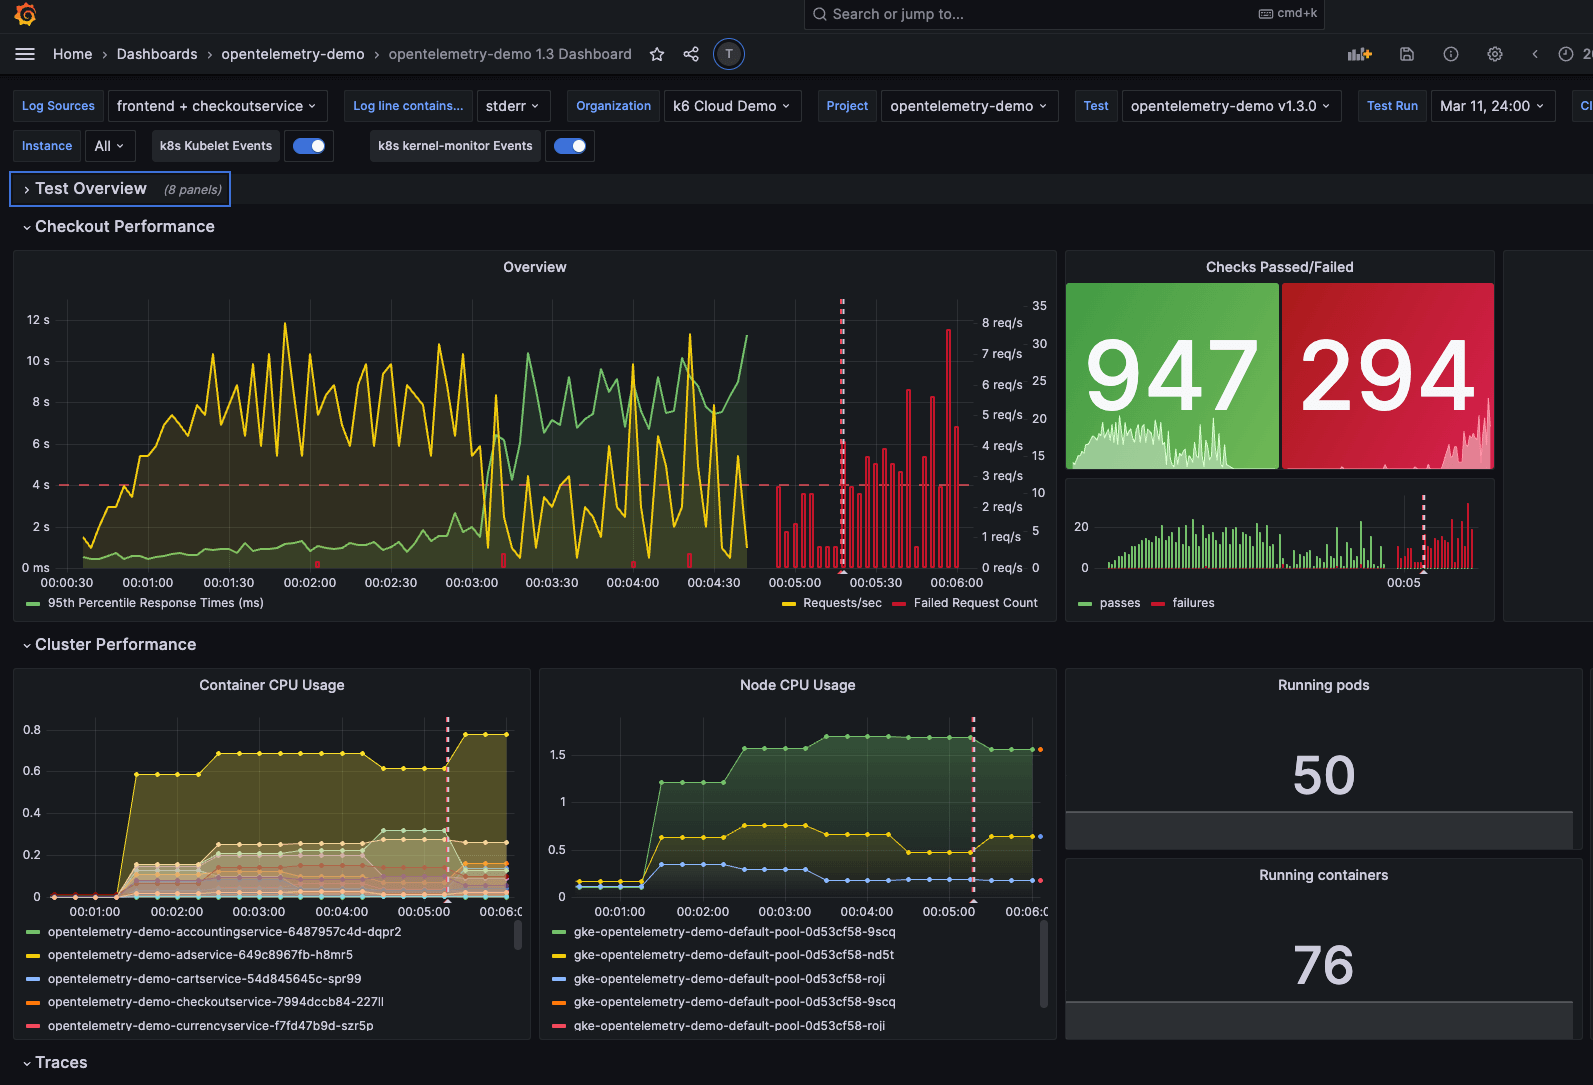
\includegraphics[scale=0.3]{assets/grafana.png}


\newpage
\section{ارزیابی}

پس از ریلیز اپلیکیشن، تیم UX مجددا از کاربر ها فیدبک گرفته و تیم پشتیبانی نرم افزار نیز به تحلیل مشکلات گزارش شده مشغول می‌شود.
پس از اینکه تمامی مشکلات جدید و ایده ها جمع آوری شد، مجددا به مرحله برنامه ریزی باز خواهیم گشت و سیستم را تا جایی که نیاز است تکامل خواهیم داد.

\newpage

\section{ابزار های استفاده شده برای این پروژه}

این پروژه کاملا بواسطه \LaTeX توسعه داده شده و از ابزار های زیر برای توسعه آن نیز استفاده شده است:

\begin{itemize}
	\item \hyperref[https://app.smartdraw.com]{https://app.smartdraw.com}
	\item \hyperref[https://app.creately.com]{https://app.creately.com}
	\item \hyperref[https://online.visual-paradigm.com/app/diagrams]{https://online.visual-paradigm.com/app/diagrams}
\end{itemize}

درضمن پروژه در مخزن و زیرپوشه زیر اکانت GitHub بنده توسعه داده شده و می‌توانید از قالب \LaTeX آن به صورت آزاد استفاده کنید.

$\hyperref[https://github.com/alirezaarzehgar/docs/tree/dev/system_analysis]{https://github.com/alirezaarzehgar/docs/tree/dev/system_analysis}$

امیدوارم این پروژه بهتون کمک کرده باشه و شما هم ازش چیزی یاد گرفته باشید XD


\end{document}
